\chapter{Diagrammes d'état}
\section{Diagramme d'état lors de l'entrée d'un utilisateur dans la salle de bain}
TODO
\begin{figure}[H]
	\centering
	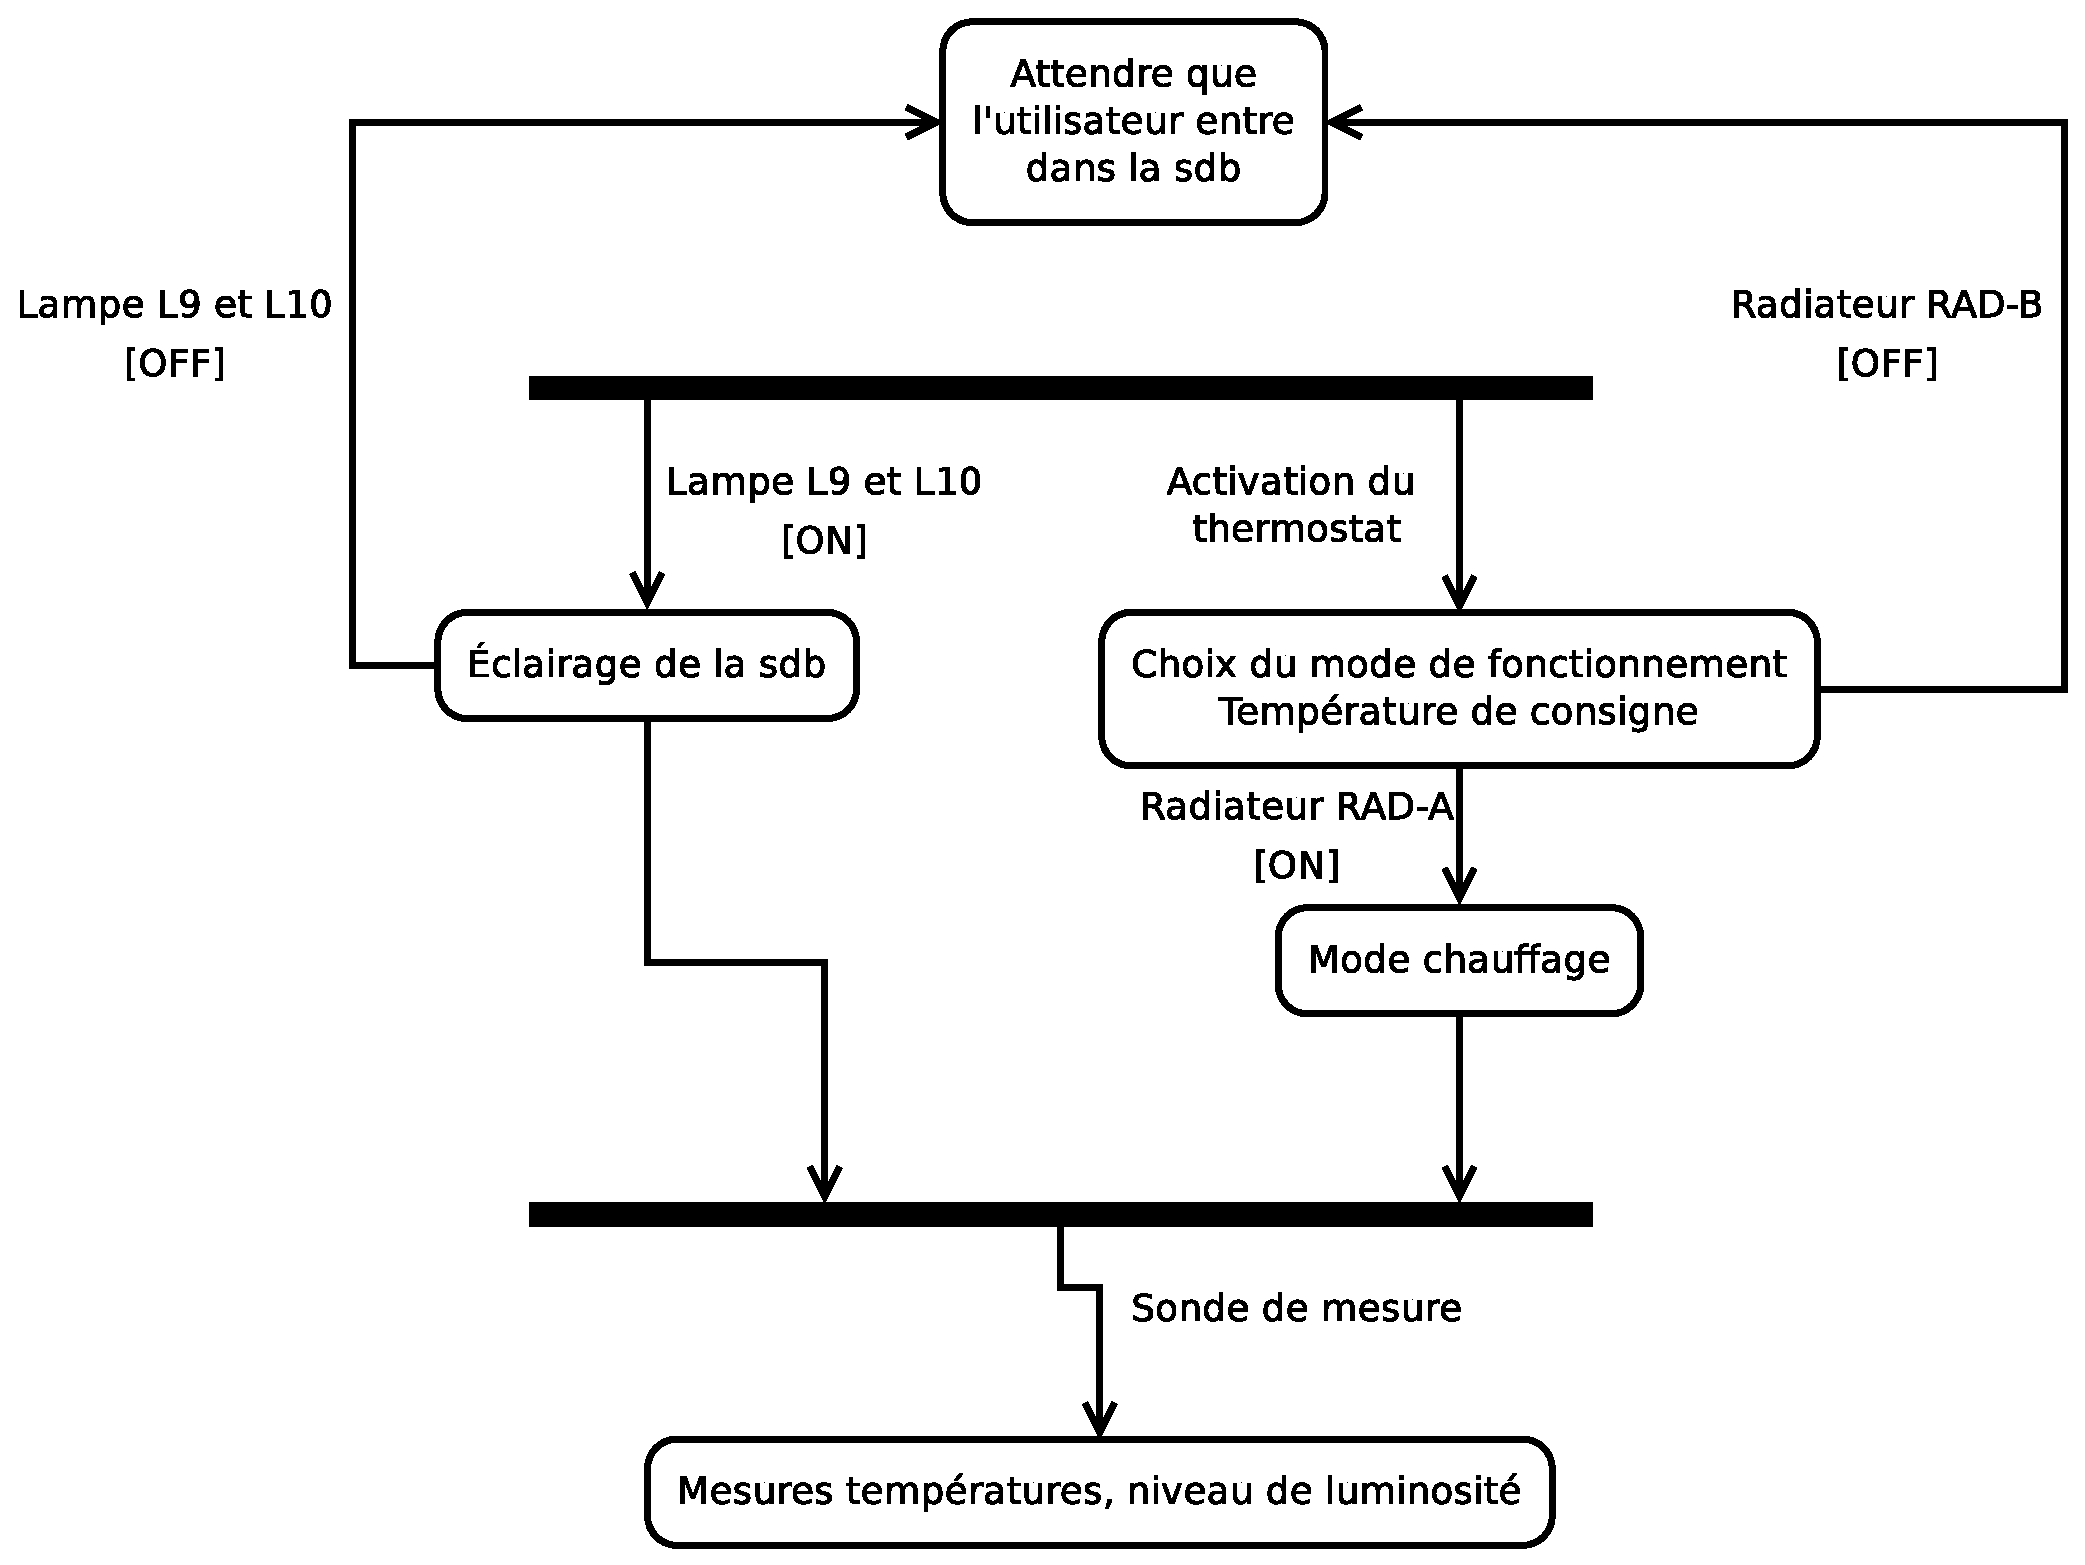
\includegraphics[width=1\linewidth]{diagrams/bathroom/diagramme_etat_st.eps}
	\caption{TODO}
	\label{fig:diagramme_st}
\end{figure}

\section{Diagramme d'état d'un utilisateur de la douche}
Le diagramme d'état ci-après décrit l'état du système lorsque l'utilisateur entre dans la douche. 

La présence de l'utilisateur dans la douche se fait au moyen d'un \textbf{capteur de charge}. Dès lors, un \textbf{capteur laser} détermine la taille de l'utilisateur afin de pouvoir adapter la hauteur de la pomme de douche à l'utilisateur. Un \textbf{capteur de position} sur le mobilier permet d'en connaître la hauteur et de la comparer à celle de l'utilisateur pour procéder à l'élévation ou l'abaissement de la dalle. 
\begin{figure}[H]
	\centering
	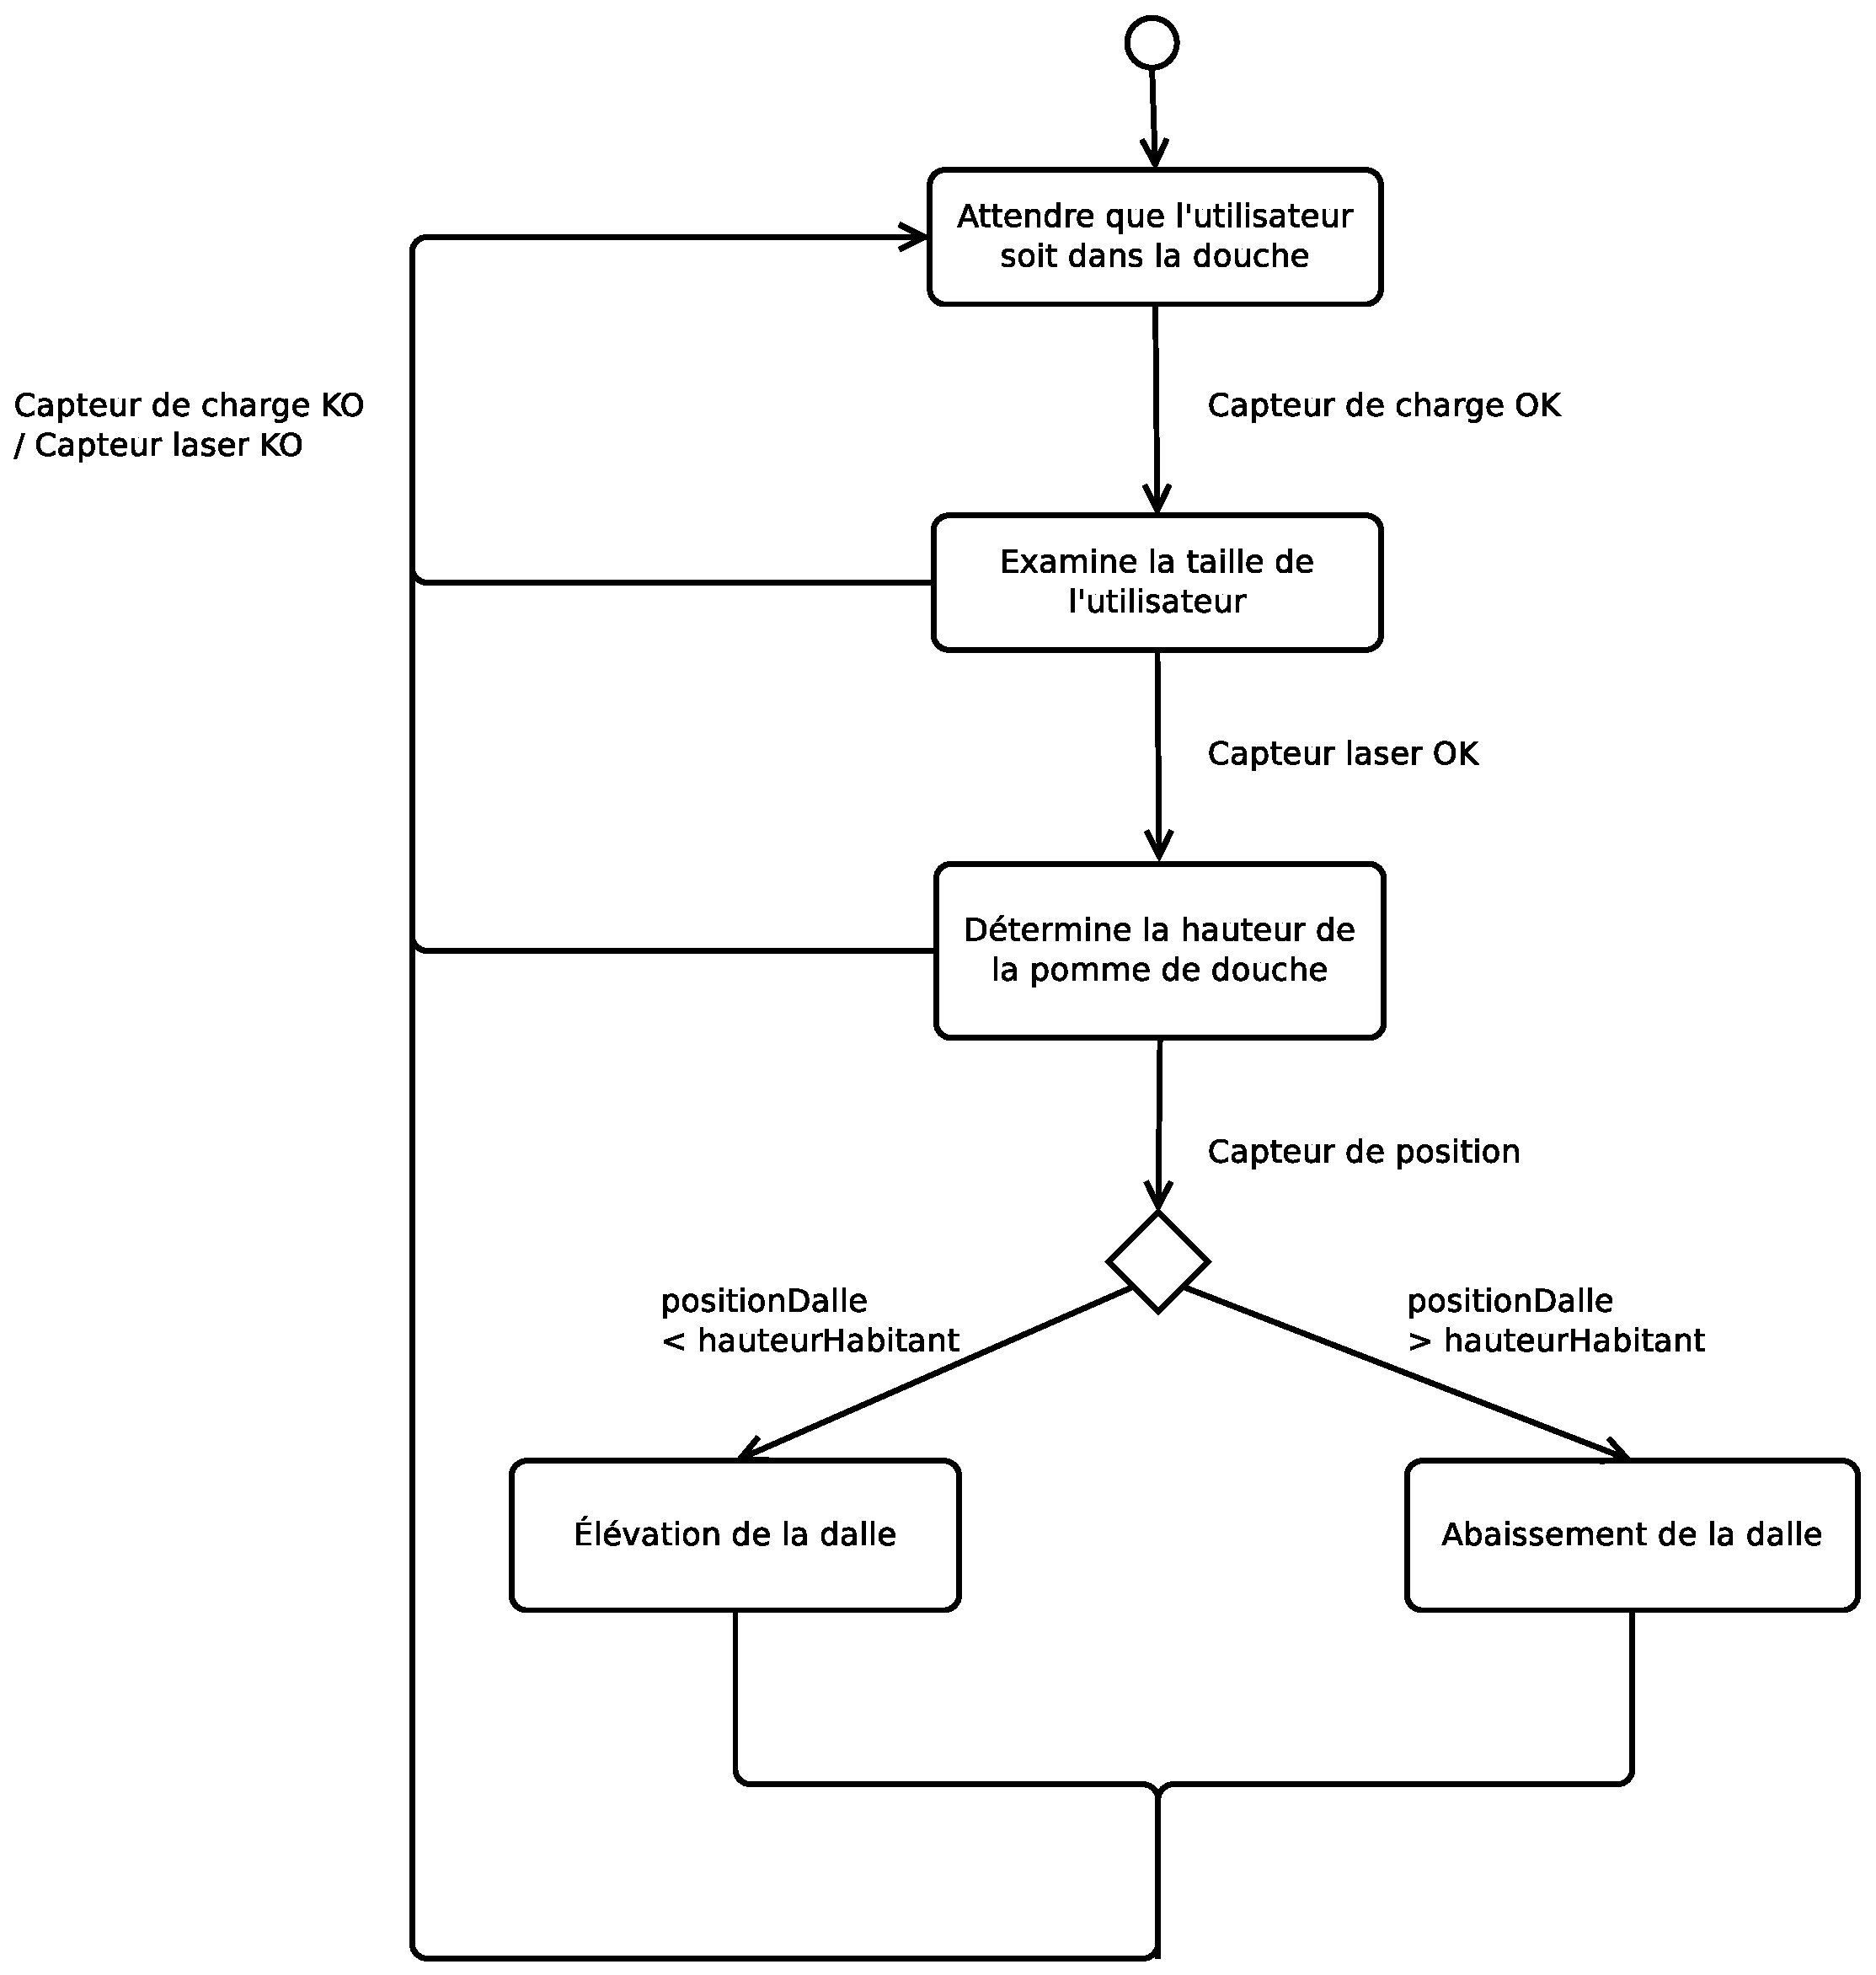
\includegraphics[width=1\linewidth]{diagrams/bathroom/diagramme_etat_st2.eps}
	\caption{Diagramme d'état d'un utilisateur de la douche}
	\label{fig:diagramme_st2}
\end{figure}
